\begin{adjustwidth*}{}{-2.25in}
\textbf{{\large Exercises}}
\setlength{\columnsep}{25pt}
\begin{multicols*}{2}
\noindent Terms and Concepts \small

\begin{enumerate}[1)]
\item {In your own words, describe what it means for a function to be continuous.}
\item {In your own words, describe what the Intermediate Value Theorem states.}
\item {What is a ``root'' of a function?}
\item {Given functions $f$ and $g$ on an interval $I$, how can the Bisection Method be used to find a value $c$ where $f(c) = g(c)$?}
\item {T/F:	If $f$ is defined on an open interval containing $c$, and $\ds \lim_{x\to c}f(x)$ exists, then $f$ is continuous at $c$.}
\item {T/F: If $f$ is continuous at $c$, then $\ds \lim_{x\to c}f(x)$ exists.}
\item {T/F: If $f$ is continuous at $c$, then $\ds \lim_{x\to c^+}f(x) = f(c)$.}
\item {T/F: If $f$ is continuous on $[a,b]$, then $\ds\lim_{x\to a^-}f(x) = f(a)$.}
\item {T/F: If $f$ is continuous on $[0,1)$ and $[1,2)$, then $f$ is continuous on $[0,2)$.}
\item {T/F: The sum of continuous functions is also continuous.}
\end{enumerate} 

\noindent {\normalsize Problems\\} \small

\noindent In exercises 11--17, a graph of $f$ is given along with a value $a$.  Determine if $f$ is continuous at $a$; if it is not, state why it is not.

\begin{enumerate}[1),resume]
\item
{\noindent $a = 1$

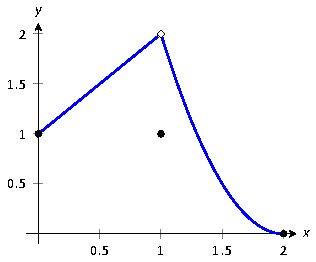
\includegraphics[scale=.8]{figures/fig01_04_ex_05}
}

\item
{\noindent $a = 1$

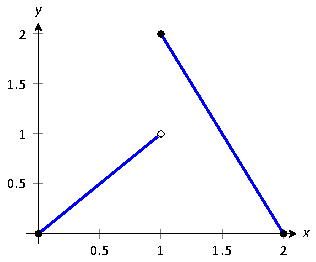
\includegraphics[scale=.8]{figures/fig01_04_ex_06}
}

\vspace{.5cm}

\item
{\noindent $a = 1$

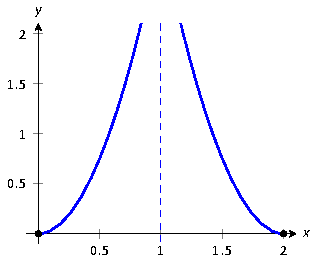
\includegraphics[scale=.8]{figures/fig01_04_ex_07}
}

\item
{\noindent $a = 0$

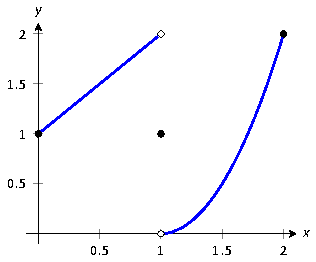
\includegraphics[scale=.8]{figures/fig01_04_ex_08}
}

\item
{\noindent $a = 1$

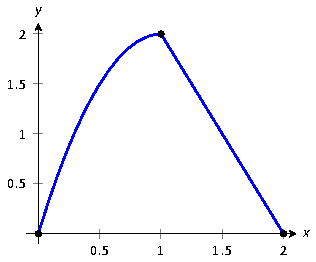
\includegraphics[scale=.8]{figures/fig01_04_ex_09}
}

\item
{\noindent $a = 4$

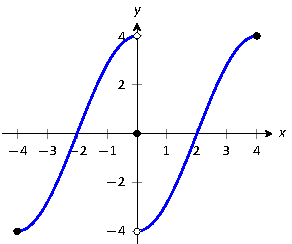
\includegraphics[scale=.8]{figures/fig01_04_ex_10}
}

\item
{\begin{enumerate}
\item		$a = -2$
\item		$a=0$
\item		$a=2$
\end{enumerate}

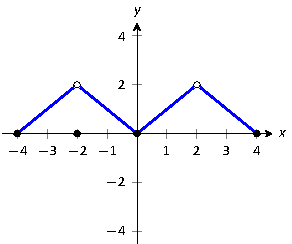
\includegraphics[scale=.8]{figures/fig01_04_ex_11}
}

\end{enumerate}

\vspace{.5cm}

%------------------------------------------
% END OF EXERCISES ON FIRST PAGE
%------------------------------------------
\end{multicols*}
\end{adjustwidth*}

\clearpage

\begin{adjustwidth*}{}{-2.25in}
\setlength{\columnsep}{25pt}
\begin{multicols*}{2}\small

In exercises 18--21, determine if $f$ is continuous at the indicated values.  If not, explain why.

\begin{enumerate}[1),start=18]
\item 
{$\ds f(x) = \left\{\begin{array}{ccc} 
1		& & x=0\\
\ds\frac{\sin(x)}{x} & & x>0
\end{array}\right.
$
\begin{enumerate}
\item		$x=0$
\item		$x=\pi$
\end{enumerate}
}

\item 
{$\ds f(x) = \left\{\begin{array}{ccc} 
x^3-x		& & x<1\\
x-2 & & x\geq 1
\end{array}\right.
$
\begin{enumerate}
\item		$x=0$
\item		$x=1$
\end{enumerate}
}

\item 
{$\ds f(x) = \left\{\begin{array}{ccc} 
\ds\frac{x^2+5x+4}{x^2+3x+2}		& &  x\neq -1\\
3 & & x=-1
\end{array}\right.
$
\begin{enumerate}
\item		$x=-1$
\item		$x=10$
\end{enumerate}
}

\item
{$\ds f(x) = \left\{\begin{array}{ccc}
\ds\frac{x^2-64}{x^2-11 x+24}		& &  x\neq 8\\
5 & & x=8
\end{array}\right.
$
\begin{enumerate}
\item		$x=0$
\item		$x=8$
\end{enumerate}
}
\end{enumerate}

\vspace{.5cm}

\noindent In exercises 22--32, give the intervals on which the given function is continuous.

\begin{enumerate}[1),start=22]
\item $\ds f(x) = x^2-3x+9$
\item $\ds g(x) = \sqrt{x^2-4}$
\item $\ds h(k) = \sqrt{1-k}+\sqrt{k+1}$
\item $\ds f(t) = \sqrt{5t^2-30}$
\item $\ds g(t) = \frac{1}{\sqrt{1-t^2}}$
\item $\ds g(x) = \frac{1}{1+x^2}$
\item $\ds f(x) = e^x$
\item $\ds g(s) = \ln s$
\item $\ds h(t) = \cos(t)$
\item $\ds f(k) = \sqrt{1-e^k}$
\item $\ds f(x) = \sin(e^x+x^2)$
\end{enumerate}

\vspace{.5cm}

\noindent In exercises 33--34, use the Bisection Method to approximate, accurate to two decimal places, the value of the root of the given function in the given interval.

\begin{enumerate}[1),start=33]
\item $\ds f(x) = \sin(x) - \frac{1}{2}; \quad [0.5, 0.55]$
\item $\ds f(x) = \cos(x) - \sin(x); \quad [0.7, 0.8]$
\end{enumerate}

%---------------------------------------------
% END OF EXERCISES ON SECOND PAGE
%---------------------------------------------
\end{multicols*}
\end{adjustwidth*}
\afterexercises